\documentclass[11pt]{article}
	\usepackage[T1]{fontenc}
    % Nicer default font (+ math font) than Computer Modern for most use cases
    % \usepackage{mathpazo}

    % Basic figure setup, for now with no caption control since it's done
    % automatically by Pandoc (which extracts ![](path) syntax from Markdown).
    \usepackage{graphics}
    % We will generate all images so they have a width \maxwidth. This means
    % that they will get their normal width if they fit onto the page, but
    % are scaled down if they would overflow the margins.
    \makeatletter
    \def\maxwidth{\ifdim\Gin@nat@width>\linewidth\linewidth
    \else\Gin@nat@width\fi}
    \makeatother
    \let\Oldincludegraphics\includegraphics
    % Set max figure width to be 80% of text width, for now hardcoded.
    \renewcommand{\includegraphics}[1]{\Oldincludegraphics[width=.8\maxwidth]{#1}}
    % Ensure that by default, figures have no caption (until we provide a
    % proper Figure object with a Caption API and a way to capture that
    % in the conversion process - todo).
    \usepackage[center,bf]{caption}
    % \DeclareCaptionLabelFormat{nolabel}{}
    % \captionsetup{labelformat=nolabel}

    \usepackage{adjustbox} % Used to constrain images to a maximum size 
    \usepackage{xcolor} % Allow colors to be defined
    \usepackage{enumerate} % Needed for markdown enumerations to work
    \usepackage{geometry} % Used to adjust the document margins
    \usepackage{amsmath} % Equations
    \usepackage{amssymb} % Equations
    \usepackage{textcomp} % defines textquotesingle
    % Hack from http://tex.stackexchange.com/a/47451/13684:
    \AtBeginDocument{%
        \def\PYZsq{\textquotesingle}% Upright quotes in Pygmentized code
    }
    \usepackage{upquote} % Upright quotes for verbatim code
    \usepackage{eurosym} % defines \euro
    \usepackage[mathletters]{ucs} % Extended unicode (utf-8) support
    \usepackage[utf8x]{inputenc} % Allow utf-8 characters in the tex document
    \usepackage{fancyvrb} % verbatim replacement that allows latex
    \usepackage{grffile} % extends the file name processing of package graphics 
                         % to support a larger range 
    % The hyperref package gives us a pdf with properly built
    % internal navigation ('pdf bookmarks' for the table of contents,
    % internal cross-reference links, web links for URLs, etc.)
    \usepackage{hyperref}
    \usepackage{longtable} % longtable support required by pandoc >1.10
    \usepackage{booktabs}  % table support for pandoc > 1.12.2
    \usepackage[inline]{enumitem} % IRkernel/repr support (it uses the enumerate* environment)
    \usepackage[normalem]{ulem} % ulem is needed to support strikethroughs (\sout)
                                % normalem makes italics be italics, not underlines
   	\usepackage[]{authblk}
   	\usepackage{cite}
    \usepackage{graphicx}
    \usepackage{hyperref}
    \usepackage{amsmath}
    \usepackage{amsthm}
    \usepackage{amssymb}
    \usepackage{bm}
    \usepackage{bbm}
    \usepackage{algorithmicx}
    \usepackage{algorithm}
    \usepackage{algpseudocode}
    \usepackage{array}
    \usepackage{booktabs}
    \usepackage{multirow}
    \usepackage{makecell}
    \usepackage{color}
    \usepackage{tabularx,ragged2e,booktabs,caption}
    \usepackage{verbatim}
   	\makeatletter
    \def\@maketitle{%
    \newpage
      \null
      \vskip 2em%
      \begin{center}%
      \let \footnote \thanks
        {\Large\bfseries \@title \par}%
        \vskip 1.5em%
        {\normalsize
          \lineskip .5em%
          \begin{tabular}[t]{c}%
            \@author
          \end{tabular}\par}%
        \vskip 1em%
        {\normalsize \@date}%
      \end{center}%
      \par
      \vskip 1.5em}
    \makeatother


\newtheorem{theorem}{Theorem}






\title{EE 232E Project 3\\Reinforcement Learning and Inverse Reinforcement Learning}
\author{Hengjie~Yang, Sheng~Chang, Wandi~Cui, and Tianyi~Liu
}


\date{\today}


\begin{document}
\maketitle

% \section{A brief tutorial on how to use this template}
% \Large\textcolor{red}{\bf{Please remove the tutorial section in the final manuscript\\ by commenting, i.e. $\%(something)$}}


% \subsection{Figures}
% Figure insertion is shown in Fig \ref{example_fig}.
% \begin{figure}[h]
% \centering
% \scalebox{0.7}{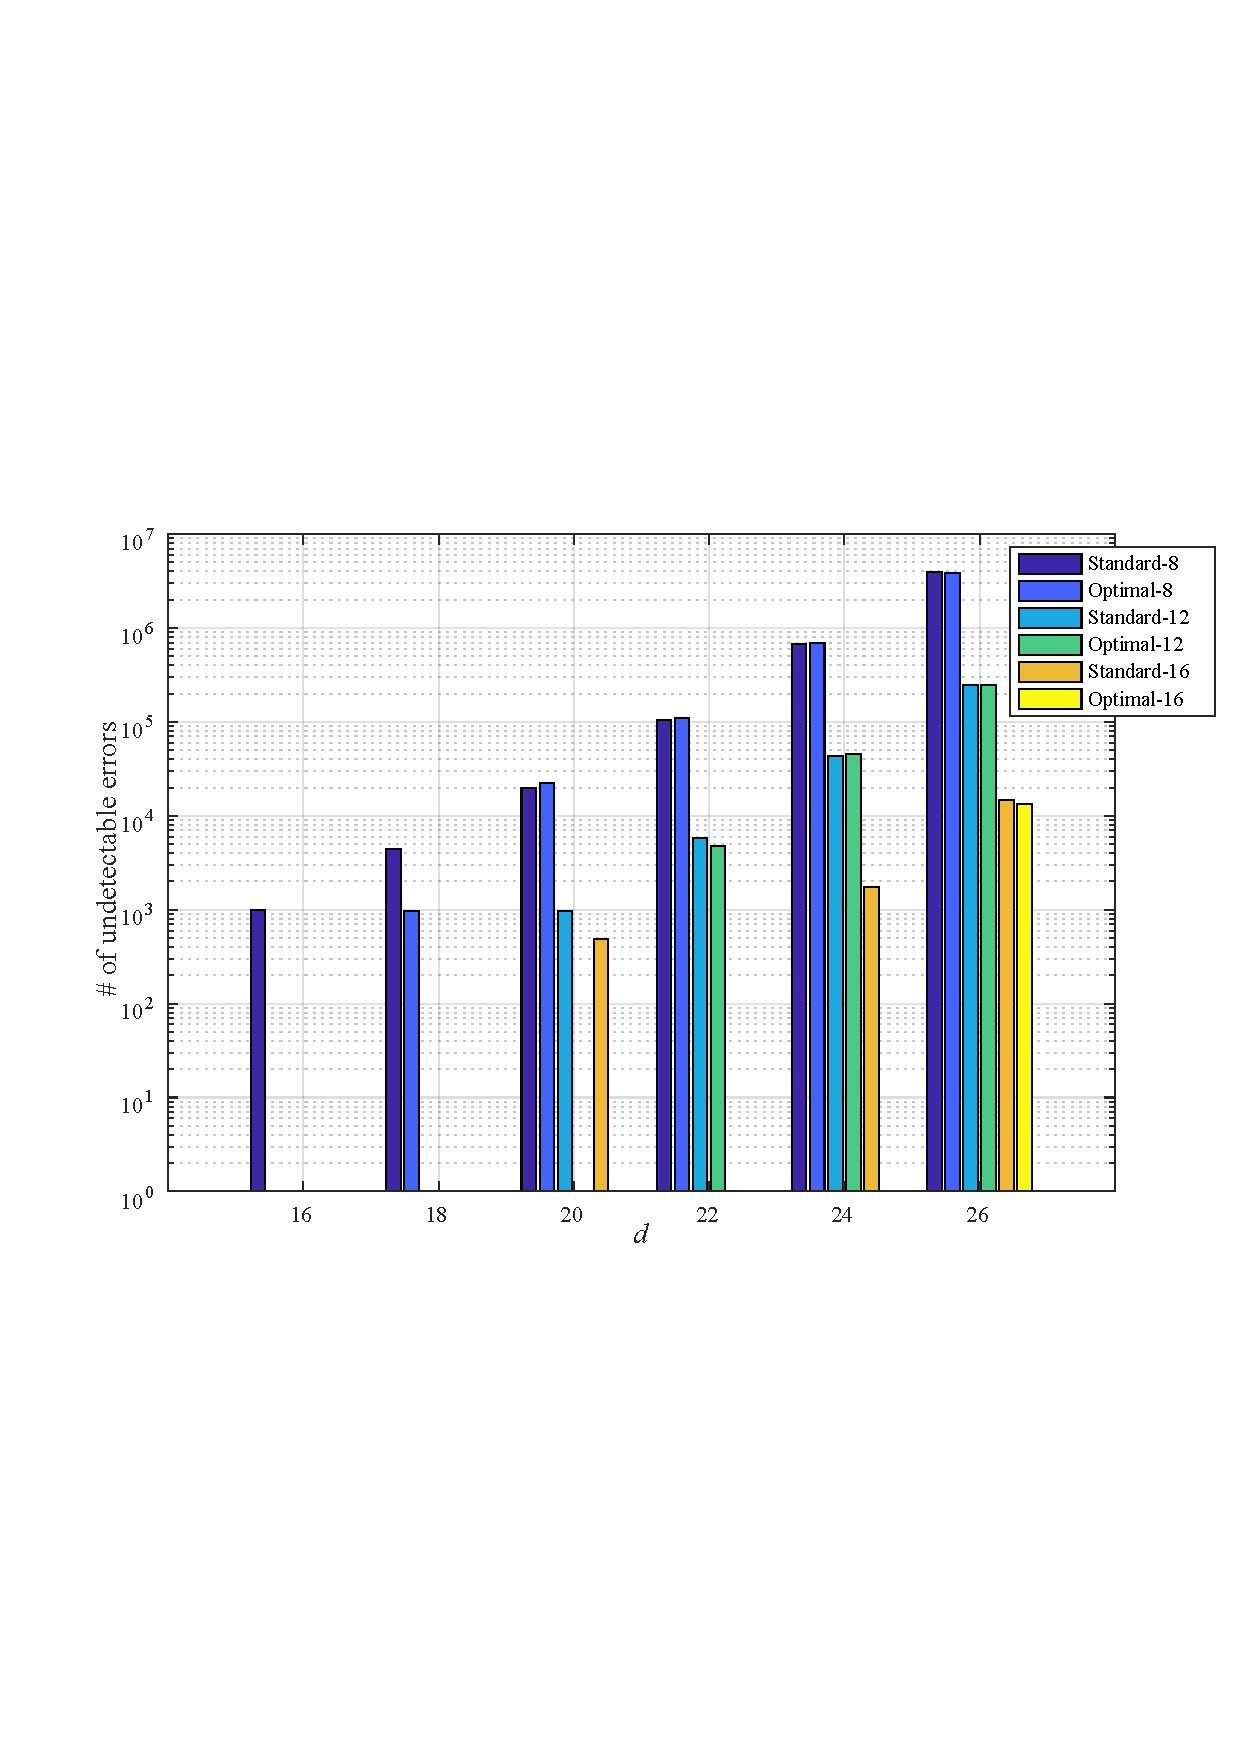
\includegraphics{Figures/spectrum_bar.pdf}}
% \caption{An example of figure insertion}
% \label{example_fig}
% \end{figure}

% \subsection{Equations}
% An example of equations is given as follows.
% \begin{theorem}
% Let $a$, $b$, $c$ denote the sides of a triangle, respectively. If $a\perp b$, the pythagoras theorem is given as follows.
% \begin{align}
% c^2 = a^2 + b^2
% \end{align}
% \end{theorem}

% \subsection{Tables}
% An example of tables is shown in Table \ref{example_table}.
% \renewcommand\arraystretch{1.1}
% \begin{table}[h]
% \center
% \caption{Standard CRC Codes versus Optimal CRC Codes for Convolutional Code $G=(561~753)$ with $n=504$ Bits}
% \scalebox{0.9}{
% \begin{tabular}{r|c|c|cccccc}
% \hline
% \multirow{2}{*}{Name} & \multirow{2}{*}{Gen. Poly.} & \multicolumn{7}{c}{Undetected Error Distance Spectrum} \\
% \cline{3-9}
%  & & $d$ & 16 & 18 & 20 & 22 & 24 & 26 \\\hline\hline
% Standard-8 & \multicolumn{1}{l}{0x19B} & & 983 & 4387 & 19909 & 105000 & 672724 & 3972970\\
% Optimal-8 & \multicolumn{1}{l}{0x19D} & & 0 & 979 & 22349 & 111304 & 686314 & 3830340\\\hline
% Standard-12 & \multicolumn{1}{l}{0x180F} & & 0 & 0 & 969 & 5815 & 42893 & 245211 \\
% Optimal-12 & \multicolumn{1}{l}{0x108B} & & 0 & 0 & 0 & 4793 & 45795 & 246729\\\hline
% Standard-16 & \multicolumn{1}{l}{0x11021} & & 0 & 0 & 484 & 0 & 1765 & 14752\\
% Optimal-16 & \multicolumn{1}{l}{0x1F8FD} & & 0 & 0 & 0 & 0 & 0 & 13240\\\hline
% \end{tabular}}
% \label{example_table}
% \end{table}




\section{Reinforcement Learning (RL)}

\begin{figure}
\centering
\begin{minipage}[h]{0.48\textwidth}
\centering
\scalebox{1}{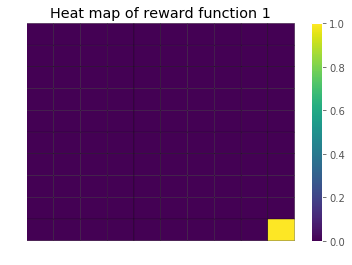
\includegraphics{Figures/hj_01.png}}
\caption{Heat map of reward function $1$}
\label{fig:hm_reward_1}
\end{minipage}
\begin{minipage}[h]{0.48\textwidth}
\centering
\scalebox{1}{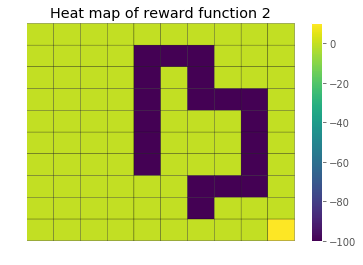
\includegraphics{Figures/hj_02.png}}
\caption{Heat map of reward function $2$}
\label{fig:hm_reward_2}
\end{minipage}
\end{figure}

In this project, we implement the RL algorithm to explore its performance. 

\textcolor{red}{Question 1: (10 points) For visualization purpose, generate heat maps of Reward function 1 and Reward function 2. For the heat maps, make sure you display the coloring scale. You will have 2 plots for this question}

The heat map of reward function $1$ and $2$ are plotted in Fig. \ref{fig:hm_reward_1}  and \ref{fig:hm_reward_2}, respectively.


\subsection{Optimal policy learning using RL algorithms}

\textcolor{red}{Question 2: (40 points) Create the environment of the agent using the information provided in section 2. To be specific, create the MDP by setting up the state-space, action set, transition probabilities, discount factor, and reward
function. For creating the environment, use the following set of parameters:}
\begin{itemize}
\item Number of states = $100$ (state space is a 10 by 10 square grid as displayed
in figure 1)
\item Number of actions = $4$ (set of possible actions is displayed in figure 2)
\item $w = 0.1$
\item Discount factor $\gamma = 0.8$
\item Reward function $1$
\end{itemize}

\textcolor{red}{
    After you have created the environment, then write an optimal state-value function that takes as input the environment of the agent and outputs the optimal value of each state in the grid. For the optimal state-value function, you have to implement the Initialization (lines 2-4) and Estimation (lines 5-13) steps of the Value Iteration algorithm. For the estimation step, use $\epsilon=0.01$. For visualization purpose, you should generate figure similar to that of figure 1 but with the number of state replaced by the optimal value of that state. In this question, you should have 1 plot.
}

After implementing the RL algorithm, we obtain the grid of optimal state values in Fig. \ref{fig:optimal_state_value_01}.


\begin{figure}
\centering
\begin{minipage}[t]{0.48\textwidth}
\centering
\scalebox{1}{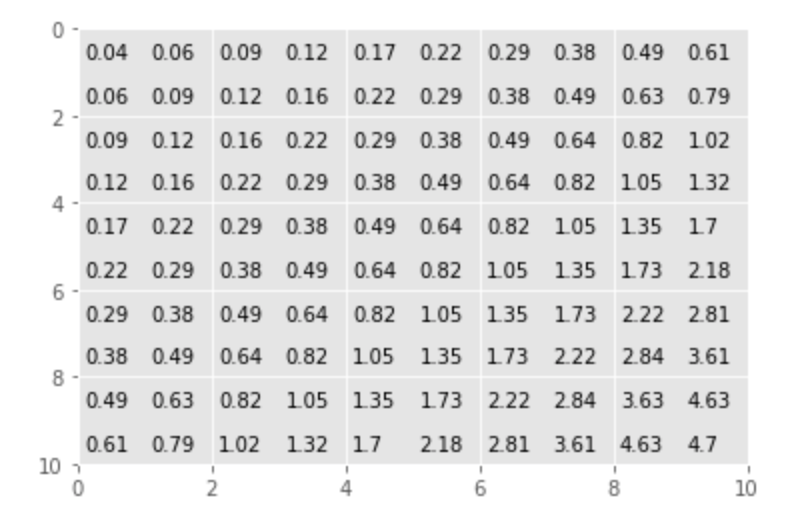
\includegraphics{Figures/r1_val_map.png}}
\caption{The optimal state value with reward function $1$}
\label{fig:optimal_state_value_01}
\end{minipage}
\begin{minipage}[t]{0.48\textwidth}
\centering
\scalebox{1}{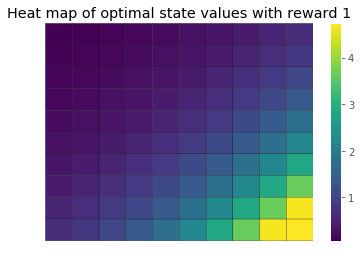
\includegraphics{Figures/hj_04.png}}
\caption{Heat map of optimal state values with reward function $1$}
\label{fig:hm_opt_state_value_01}
\end{minipage}
\end{figure}
\vspace{10pt}

\textcolor{red}{
    Question 3: (5 points) Generate a heat map of the optimal state values across the 2-D grid. For generating the heat map, you can use the same function provided in the hint earlier (see the hint after question 1).
}

After obtaining the optimal state value array with reward function $1$, the corresponding heat map of it is shown in Fig. \ref{fig:hm_opt_state_value_01}.
\vspace{10pt}

\textcolor{red}{
    Question 4: (15 points) Explain the distribution of the optimal state values across the 2-D grid. (Hint: Use the figure generated in question 3 to explain)
}

Since we observe from reward function $1$ that the reward function is symmetric with respect to the diagonal. So according to the RL algorithm, it follows that the optimal state value should also be symmetric with respect to the diagonal. Also, the value increases as they become close to the $(9,9)$ state.
\vspace{10pt}

\textcolor{red}{
    Question 5: (30 points) Implement the computation step of the value iteration algorithm (lines 14-17) to compute the optimal policy of the agent navigating
the 2-D state-space. For visualization purpose, you should generate a figure similar to that of figure 1 but with the number of state replaced by the optimal action at that state. The optimal actions should be displayed using arrows. Does the optimal policy of the agent match your intuition? Please provide a brief explanation. Is it possible for the agent to compute the optimal action to take at each state by observing the optimal values of it's neighboring states? In this question, you should have 1 plot.
}

\begin{figure}
\centering
\begin{minipage}[t]{0.48\textwidth}
\centering
\scalebox{1}{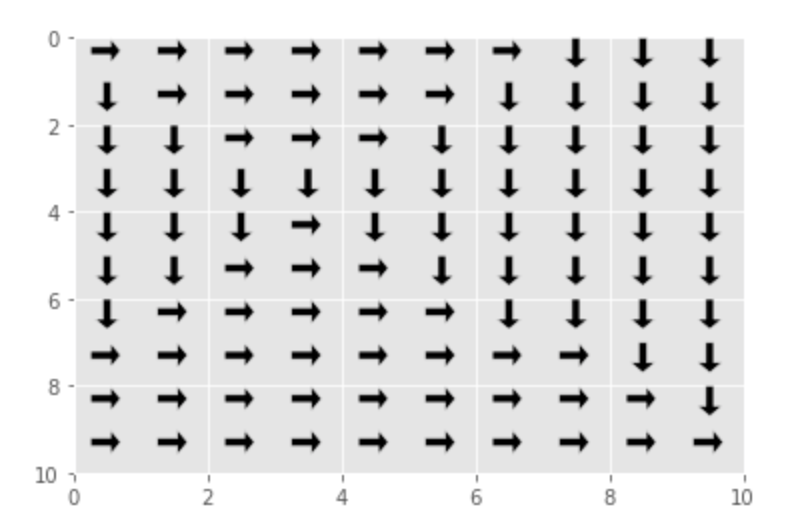
\includegraphics{Figures/r1_policy_map.png}}
\caption{Optimal actions with reward function $1$}
\label{fig:opt_action_01}
\end{minipage}
\begin{minipage}[t]{0.48\textwidth}
\centering
\scalebox{1}{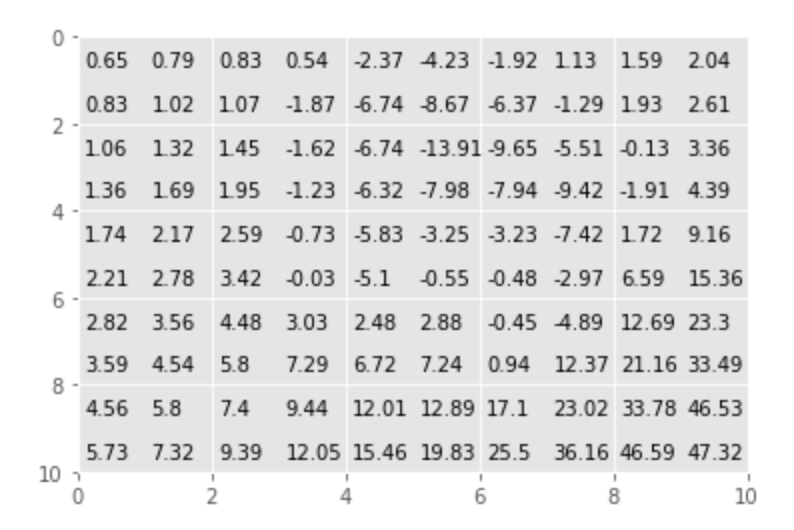
\includegraphics{Figures/r2_val_map.png}}
\caption{The optimal state value with reward function $2$}
\label{fig:opt_state_value_02}
\end{minipage}
\end{figure}

After implementing the computation step, the optimal actions at each state are shown in Fig. \ref{fig:opt_action_01}. The optimal policy of the agent matches the intuition since the action is always towards the highest score. Yes, the optimal action is always towards the neighbor with the highest state value. Therefore, we can determine the optimal action by simply observing the values in the neighboring states.
\vspace{10pt}

\textcolor{red}{
    Question 6: (10 points) Modify the environment of the agent by replacing Reward function 1 with Reward function 2. Use the optimal state-value function implemented in question 2 to compute the optimal value of each state in the grid. For visualization purpose, you should generate a figure similar to that of figure 1 but with the number of state replaced by the optimal value of that state. In this question, you should have 1 plot.
}


After replacing with reward function $2$, the optimal value at each state is shown in Fig. \ref{fig:opt_state_value_02}.
\vspace{10pt}

\begin{figure}
\centering
\begin{minipage}[t]{0.48\textwidth}
\centering
\scalebox{1}{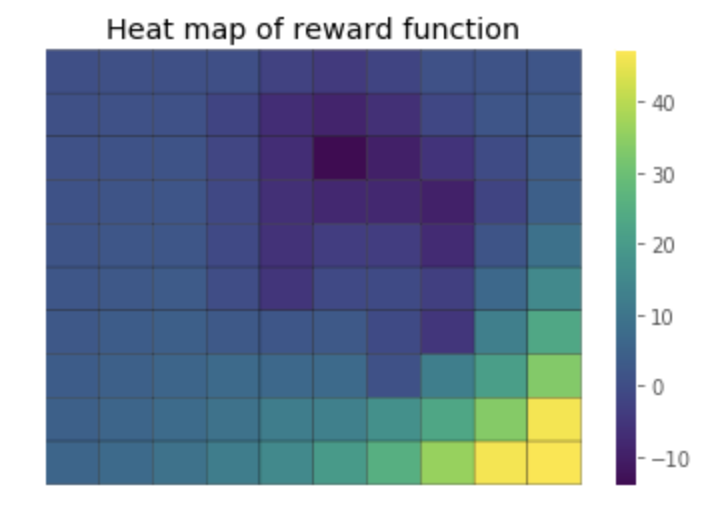
\includegraphics{Figures/r2_val_heatmap.png}}
\caption{Heat map of optimal state values with reward function $2$}
\label{fig:hm_opt_state_value_02}
\end{minipage}
\begin{minipage}[t]{0.48\textwidth}
\centering
\scalebox{1}{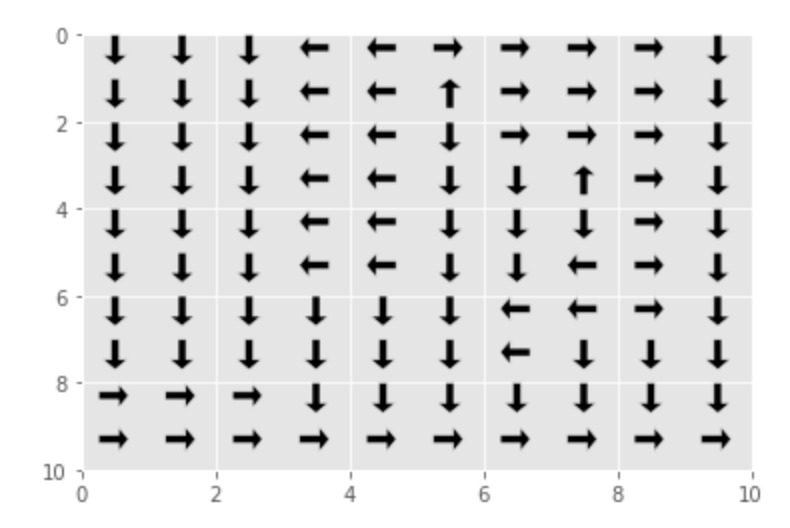
\includegraphics{Figures/r2_policy_map.png}}
\caption{Optimal actions with reward function $2$}
\label{fig:opt_actions_02}
\end{minipage}
\end{figure}

\textcolor{red}{
    Question 7: (10 points) Generate a heat map of the optimal state values (found in question 6) across the 2-D grid. For generating the heat map, you can use the same function provided in the hint earlier.
}

The heat map of the optimal state values is shown in Fig. \ref{fig:hm_opt_state_value_02}.
\vspace{10pt}

\textcolor{red}{
    Question 8: (20 points) Explain the distribution of the optimal state values across the 2-D grid. (Hint: Use the figure generated in question 7 to explain)
}

The distribution of the optimal state values is that, in the area with the reward score of $-100$, the optimal state values are zero. In the area with the reward score of $0$, the optimal state values are positive, and are increasing as they become close to the $(9,9)$ state which has the highest reward score of $10$. The $(9,9)$ state has the highest state value as it has the highest reward score.

\textcolor{red}{
    Question 9: (20 points) Implement the computation step of the value iteration algorithm (lines 14-17) to compute the optimal policy of the agent navigating the 2-D state-space. For visualization purpose, you should generate a figure
similar to that of figure 1 but with the number of state replaced by the optimal action at that state. The optimal actions should be displayed using arrows. Does the optimal policy of the agent match your intuition? Please provide a
brief explanation. In this question, you should have 1 plot.
}

After implementing the computation step, the optimal actions with reward function $2$ are shown in Fig. \ref{fig:opt_actions_02}. The optimal action policy matches the intuition as the actions are still towards the neighboring state with the highest state value.









\section{Inverse Reinforcement Learning (IRL)}

\subsection{IRL algorithm}

\textcolor{red}{
    Question 10: Express $c$, $x$, $D$ in terms of $R$, $P_{a}$, $P_{a_{1}}$ , $t_{i}$, $u$, $\lambda$ and $R_{max}$
}

To recast the equation into block matrices, let $T = [t_{1}, t_{2},...,t_{|s|}]^T$, $U = [u_{1}, u_{2},...,u_{|s|}]^T$, 
$R = [R(s_{1}),...,R(s_{|s|})]^T$. 

Then the cost function can be expressed as $[0, I,$$\lambda$ * $I$$, 0] * [$R$,$T$,$U$]$

$$\max\limits_{x} 
\left[
 \begin{matrix}
   0 & 1^T & -\lambda 1^T
  \end{matrix}
  \right] \left[
 \begin{matrix}
   R \\
   T \\ 
   U
  \end{matrix}
  \right] 
$$


$$ st:
\left[
 \begin{matrix}
   -(P_{a_1} - P_{a})(I- \gamma P_{a_1})^{-1}  & I & 0 \\
   -(P_{a_1} - P_{a})(I- \gamma P_{a_1})^{-1}  & 0 & 0 \\
   -I & 0 & -I \\
   I & 0 & -I \\
   I & 0 & 0 \\
   -I & 0 & 0 \\
  \end{matrix}
  \right] \left[
 \begin{matrix}
   R \\
   T \\ 
   U
  \end{matrix}
  \right] \le 
  \left[
  \begin{matrix}
   0 \\
   0 \\ 
   0 \\
   R_{max} \\
   R_{max}
  \end{matrix}
  \right]
$$
 
Thus,
$$ D = 
 \left[
 \begin{matrix}
   -(P_{a_1} - P_{a})(I- \gamma P_{a_1})^{-1}  & I & 0 \\
   -(P_{a_1} - P_{a})(I- \gamma P_{a_1})^{-1}  & 0 & 0 \\
   -I & 0 & -I \\
   I & 0 & -I \\
   I & 0 & 0 \\
   -I & 0 & 0 \\
  \end{matrix}
  \right]
$$

$$x =
\left[
 \begin{matrix}
   R \\
   T \\ 
   U
  \end{matrix}
  \right]
$$

$$c = 
\left[
 \begin{matrix}
   0 \\
   1 \\ 
   \lambda 1 \\
  \end{matrix}
  \right]
$$



\subsection{Performance measure}

\textcolor{red}{
    Question 11: (30 points) Sweep $\lambda$ from $0$ to $5$ to get $500$ evenly spaced values for $\lambda$. For each value of $\lambda$ compute $O_{A}(s)$ by following the process described above. For this problem, use the optimal policy of the agent found in question 5 to fill in the $O_{E}(s)$ values. Then use equation 3 to compute the accuracy of the IRL algorithm for this value of $\lambda$. You need to repeat the above process for all $500$ values of $λ$ to get $500$ data points. Plot $\lambda$ (x-axis) against Accuracy (y-axis). In this question, you should have 1 plot.
}

The plot of $\lambda$ against Accuracy is shown in Fig. \ref{3_1}.\\

\begin{figure}
\centering
\scalebox{0.5}{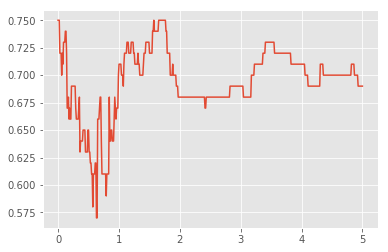
\includegraphics{Figures/3_1.png}}
\caption{The plot of Accuracy with $\lambda$}
\label{3_1}
\end{figure}

\textcolor{red}{
    Question 12: (5 points) Use the plot in question 11 to compute the value of $\lambda$ for which accuracy is maximum. For future reference we will denote this value as $\lambda_{max}$. Please report $\lambda_{max}$
}

From the plot, we can see the max accuracy is $0.75$, and there are several $\lambda$ which can reach the maximum accuracy. One of them is $1.57314$.\\

\textcolor{red}{
    Question 13: for $\lambda_{max}$, generate heat maps of the ground truth reward and the extracted reward. Please note that the ground truth reward is the Reward function 1 and the extracted reward is computed by solving the linear program given by equation 2 with the $\lambda$ parameter set to $\lambda_{max}$. In this question, you should have 2 plots.
}

The heat map of ground truth reward and extracted reward are shown in Fig. \ref{3_2_1} and Fig. \ref{3_2}, respectively.\\

\begin{figure}
\centering
\begin{minipage}[h]{0.48\textwidth}
\centering
\scalebox{1}{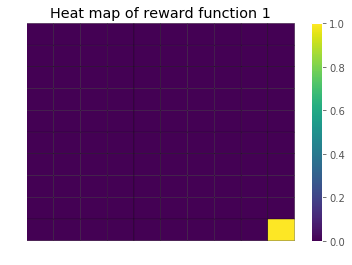
\includegraphics{Figures/hj_01.png}}
\caption{Heat map of ground truth reward}
\label{3_2_1}
\end{minipage}
\begin{minipage}[h]{0.48\textwidth}
\centering
\scalebox{1}{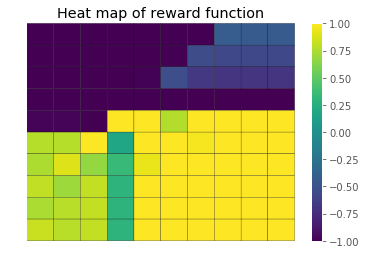
\includegraphics{Figures/3_2.png}}
\caption{Heat map of extracted reward}
\label{3_2}
\end{minipage}
\end{figure}

\textcolor{red}{
    Question 14: Use the extracted reward function computed in question 13, to compute the optimal values of the states in the 2-D grid. For computing the optimal values you need to use the optimal state-value function that you wrote in question 2. For visualization purpose, generate a heat map of the optimal state values across the 2-D grid (similar to the figure generated in question 3). In this question, you should have 1 plot.
}

The heat map of optimal values of the states computed from extracted reward function is shown in Fig. \ref{3_3}.\\

\begin{figure}
\centering
\begin{minipage}[h]{0.48\textwidth}
\centering
\scalebox{1}{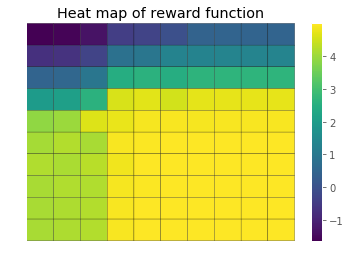
\includegraphics{Figures/3_3.png}}
\caption{The heat map of optimal values}
\label{3_3}
\end{minipage}
\begin{minipage}[h]{0.48\textwidth}
\centering
\scalebox{1}{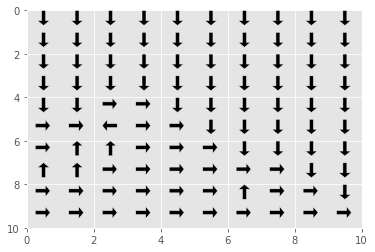
\includegraphics{Figures/3_4.png}}
\caption{The arrows plot of optimal policy}
\label{3_4}
\end{minipage}
\end{figure}

\textcolor{red}{
    Question 15: (10 points) Compare the heat maps of Question 3 and Question 14 and provide a brief explanation on their similarities and differences.
}

In comparison to heat maps of optimal values from result of the RL algorithms, the corresponding heat maps of the result of IRL algorithm has the same tendency of value distribution. We can see the top left corner's optimal values is the lowest and the bottom right corner has the highest value in both map, which is consistent with the value distribution of reward function. However, due to the difference of reward function they derived from, the result of RL algorithm has a much smoother transition from the top left corner to the bottom right corner and also is diagonal symmetric.\\

\textcolor{red}{
    Question 16: Use the extracted reward function found in question 13 to compute the optimal policy of the agent. For computing the optimal policy of the agent you need to use the function that you wrote in question 5. For visualization purpose, you should generate a figure similar to that of figure 1 but with the number of state replaced by the optimal action at that state. The actions should be displayed using arrows. In this question, you should have 1 plot.
}

The arrows plot of optimal policy computed from extracted reward function is shown in Fig. \ref{3_4}.\\

\textcolor{red}{
    Question 17: (10 points) Compare the figures of Question 5 and Question 16 and provide a brief explanation on their similarities and differences.
}

In conclusion, both figures have shown that the overall optimal policy is to make action starting from the top left corner eventually stop at the bottom right corner and most states on the right have optimal policy of going down and for states on the bottom they mostly aim to go right. On the other side, we can also that there are a few states of result of IRL algorithm has the opposite direction, which obviously is a mistake.\\

\textcolor{red}{
    Question 18: (30 points) Sweep $\lambda$ from $0$ to $5$ to get $500$ evenly spaced values for $\lambda$. For each value of $\lambda$ compute $O_{A}(s)$ by following the process described above. For this problem, use the optimal policy of the agent found in question 9 to fill in the $O_{E}(s)$ values. Then use equation 3 to compute the accuracy of the IRL algorithm for this value of λ. You need to repeat the above process for all $500$ values of $\lambda$ to get $500$ data points. Plot $\lambda$ (x-axis) against Accuracy (y-axis). In this question, you should have 1 plot.
}

The plot of $\lambda$ against Accuracy is shown in Fig. \ref{4_1}.\\

\begin{figure}
\centering
\scalebox{0.5}{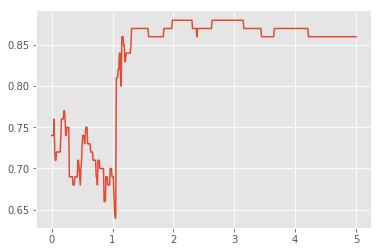
\includegraphics{Figures/4_1.png}}
\caption{The plot of Accuracy with $\lambda$}
\label{4_1}
\end{figure}

\textcolor{red}{
    Question 19: (5 points) Use the plot in question 18 to compute the value of $\lambda$ for which accuracy is maximum. For future reference we will denote this value as $\lambda_{max}$. Please report $\lambda_max{max}$
}

From the plot, we can see the max accuracy is $0.88$, and there are several $\lambda$ which can reach the maximum accuracy. One of them is $0$.\\

\textcolor{red}{
    Question 20: for $\lambda_{max}$, generate heat maps of the ground truth reward and the extracted reward. Please note that the ground truth reward is the Reward function 2 and the extracted reward is computed by solving the linear program given by equation 2 with the $\lambda$ parameter set to $\lambda_{max}$. In this question, you should have 2 plots.
}

The heat map of ground truth reward and extracted reward are shown in Fig. \ref{4_2_1} and Fig. \ref{4_2}, respectively.\\

\begin{figure}
\centering
\begin{minipage}[h]{0.48\textwidth}
\centering
\scalebox{1}{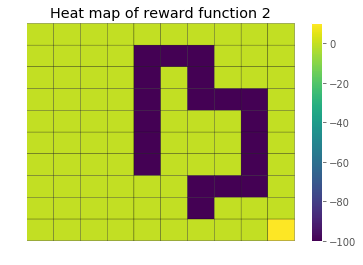
\includegraphics{Figures/hj_02.png}}
\caption{Heat map of ground truth reward}
\label{4_2_1}
\end{minipage}
\begin{minipage}[h]{0.48\textwidth}
\centering
\scalebox{1}{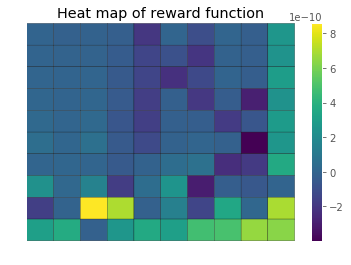
\includegraphics{Figures/4_2.png}}
\caption{Heat map of extracted reward}
\label{4_2}
\end{minipage}
\end{figure}

\textcolor{red}{
    Question 21: Use the extracted reward function computed in question 20, to compute the optimal values of the states in the 2-D grid. For computing the optimal values you need to use the optimal state-value function that you wrote in question 2. For visualization purpose, generate a heat map of the optimal state values across the 2-D grid (similar to the figure generated in question 7). In this question, you should have 1 plot.
}

The heat map of optimal values of the states computed from extracted reward function is shown in Fig. \ref{4_3}.\\

\begin{figure}
\centering
\begin{minipage}[h]{0.48\textwidth}
\centering
\scalebox{1}{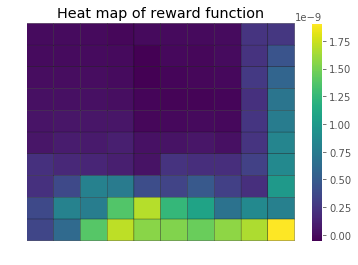
\includegraphics{Figures/4_3.png}}
\caption{The heat map of optimal values}
\label{4_3}
\end{minipage}
\begin{minipage}[h]{0.48\textwidth}
\centering
\scalebox{1}{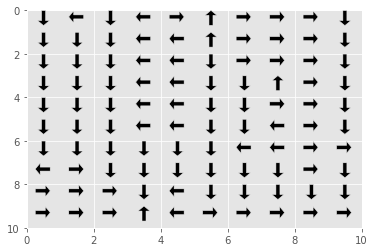
\includegraphics{Figures/4_4.png}}
\caption{The arrows plot of optimal policy}
\label{4_4}
\end{minipage}
\end{figure}

\textcolor{red}{
    Question 22: (10 points) Compare the heat maps of Question 7 and Question 21 and provide a brief explanation on their similarities and differences.
}

Similarly with the previous result, the overall value distribution on the both map is pretty close. What we can observe from both optimal values and reward function is that the lowest optimal value exist on the states which have the lowest reward function


\textcolor{red}{
    Question 23: Use the extracted reward function found in question 20 to compute the optimal policy of the agent. For computing the optimal policy of the agent you need to use the function that you wrote in question 9. For visualization purpose, you should generate a figure similar to that of figure 1 but with the number of state replaced by the optimal action at that state. The actions should be displayed using arrows. In this question, you should have 1 plot.
}

The arrows plot of optimal policy computed from extracted reward function is shown in Fig. \ref{4_4}.\\

\textcolor{red}{
    Question 24: (10 points) Compare the figures of Question 9 and Question 23 and provide a brief explanation on their similarities and differences.
}

\textcolor{red}{
    Question 25: (50 points) From the figure in question 23, you should observe that the optimal policy of the agent has two major discrepancies. Please identify and provide the causes for these two discrepancies. One of the discrepancy can be fixed easily by a slight modification to the value iteration algorithm. Perform this modification and rerun the modified value iteration algorithm to compute the optimal policy of the agent. Also, recompute the maximum accuracy after this modification. Is there a change in maximum accuracy? The second discrepancy is harder to fix and is a limitation of the simple IRL algorithm. If you can provide a solution to the second discrepancy then we will give you a bonus of $50$ points.
}

\end{document}







